\documentclass[
    floatsintext
]{article}

\usepackage{graphicx}
\usepackage{hyperref}
\usepackage{subcaption}
\usepackage{amsmath}
\usepackage[
    backend=bibtex,
%    isbn=false,
%    url=false,
%    doi=false,
%    eprint=false,
%    hyperref=false,
%    backref=false,
%    firstinits=false,
]{biblatex}
\bibliography{references}

\hypersetup{colorlinks,urlcolor=blue}
\let \shorttitle \textbf
\begin{document}

\section{Heuristics Approach}

\shorttitle{Visual Search}

In optimising the search for tool and object configurations, one could determine the regions of contact that are likely locations for good interaction.
Human subjects show an understanding of the forces generated by their actions and of the geometric constraints of the physical world.
For example, subjects performing our tool fitting tasks, examine the geometry of objects and stop at likely positions before attempting interaction.  

Tool and object configurations, bearing high likelihood of success, would satisfy two criteria: 
\begin{enumerate}
\item \textbf{Geometric constraints} of the two objects must be met. That means, the shapes of the two objects should adequately fit.
\item \textbf{Contact forces} generated must correspond to the intention of the actions executed. 
  For a lifting action, the human subject would focus on points of contact that permit vertical forces to be applied.
\end{enumerate}

The large number of possible tool and object configurations can be reduced by the above criteria. Time consuming simulations would therefore no longer be required (akin to mental simulation \cite{osiurak2014}).
As with human subjects, only potential solutions would be tested. This can be simulated through the use of a physics engine. 

\subsection{Geometric Constraints}
The geometries of the tool and object must be compatible.
In other words, either the active or passive object’s geometry must fit within the gaps and edges of its counterpart.
It is not necessary for the whole geometries to fit.  
If the tool's functional part match the gaps of the passive object, then the configuration is likely to achieve the user's intended effect. 

Tighter fits, offer better transfer of energy and control over movement.
A good fit would therefore require less manipulation effort.
In the paradigm of 4CT \cite{osiurak2014}, the effort constraint would explain why users prefer one tool fitting solution over another. 
To find parts that provide tighter fits, we consider techniques of shape similarity in matching object parts.

\subsubsection{Shape Description and Matching Techniques}
Shape analysis techniques have traditionally been engaged in image processing and computer vision for detecting and tracking objects of similar features \cite{loncaric1998,zhang2004,robert2012}.
The last two decades have provided many approaches for this type of problem \cite{loncaric1998,zhang2004,veltkamp2001,robert2012}.
Fundamentally, shape analysis is used in detecting similarity even as objects undergo geometric transformations of rotation, translation, scaling, or shearing (fig. \ref{fig:affine_transform}).

\begin{figure}[h]
  \centering
  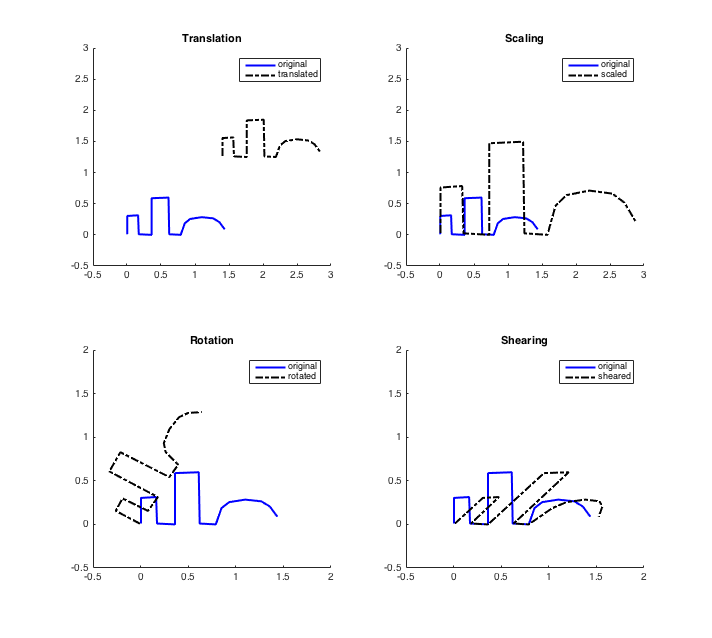
\includegraphics[width=1\textwidth]{./figures/affine_transform.png}
  \caption{Graphical examples of affine transformations}
  \label{fig:affine_transform}
\end{figure}  .     

\cite{zhang2004} distinguishes two types of techniques: contour-based and region-based.
These are further divided into structural and global approaches.
Figure \ref{fig:shape_similarity} shows a comprehensive classification of prominent shape analysis techniques. 

\begin{figure}[h]
  \centering
  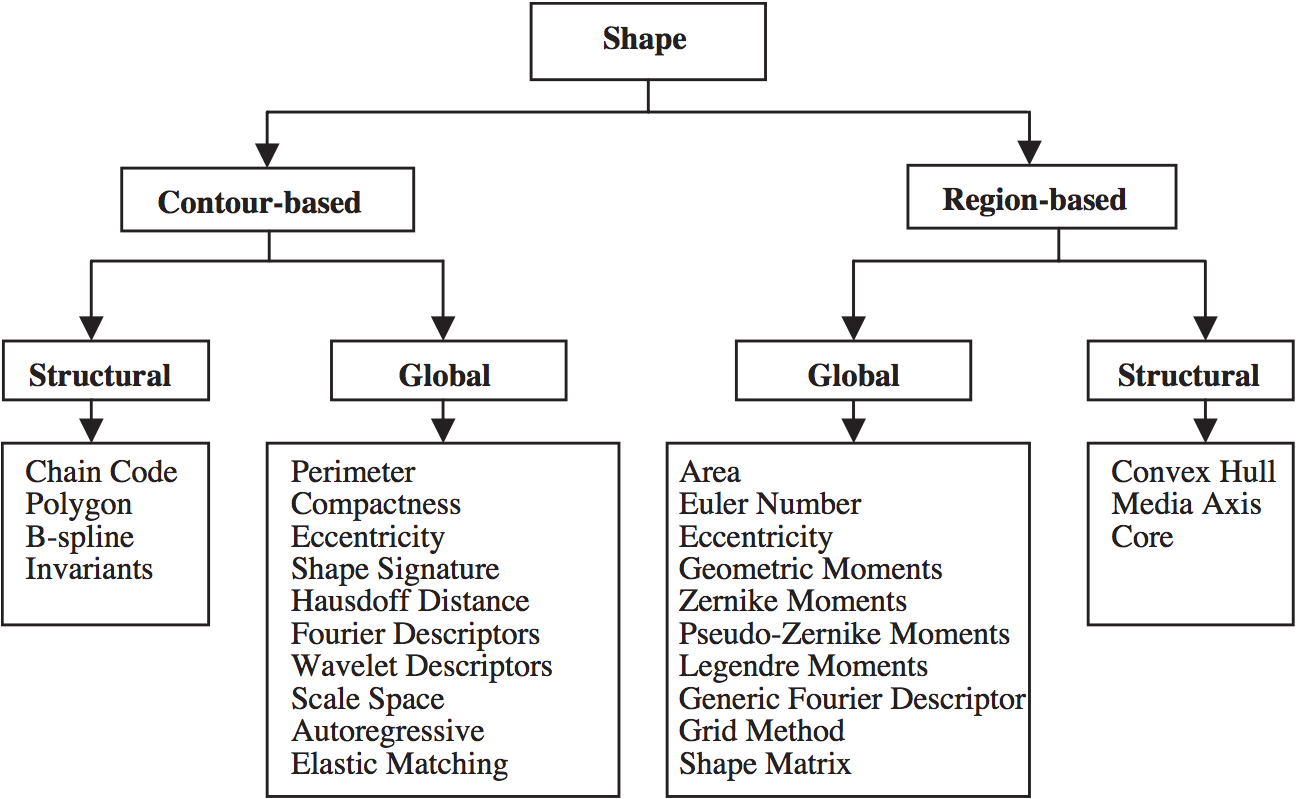
\includegraphics[width=1\textwidth]{./figures/similarity_techniques.png}
  \caption{Classification of shape similarity techniques (reprinted from \cite{zhang2004})}
  \label{fig:shape_similarity}
\end{figure}  

Contour-based techniques assesses similarity by extracting features from the object's edge.
In comparison, region techniques work by assessing surface level information such as: colour, gradient changes and surface medial.
Techniques from both approaches have justification in human perception \cite{chatbri2016}.
Nonetheless, our context excludes region-based approaches as tool parts must correspond to object gaps.
Gaps however do not contain surface information. 

In structural approaches, shapes are considered to be composed out of primitives. For contour techniques these primitives are line segments on the boundary of an object.
Primitives can be organised as either linear list of segments (\cite{zhang2004}), or as tree like structures that carry hierarchical information (\cite{zhu2015}).
In structural approaches, two objects are considered similar when they have the same primitive composition.
As comparison, global approaches make use of shapes as a whole when assessing similarity. 

Both structural and global approaches have justification in human perception \cite{zhang2004}.
Human subjects show a preference for features even when other shape descriptors are available \cite{chatbri2016}.
At the same time, global shape perception seems to precede local feature detection \cite{navon1977}. 
For that reason, both global and structural approaches should be considered. 

Correctly mimicking human behaviour would require more insight into human visual perception.
\cite{loncaric1998} describes several theories of human perception, but with an emphasis on image processing.
In a tool use scenario, emphasis should be given to theories describing perception as volumetric, as through the use of generalised cylinders \cite{dickinson2014}.
Such theories may better explain human tool ability and can be explored in future work.    

\subsubsection{Limitations}
As previously remarked, contour-based techniques contain promising approaches in solving tool-object fitting problems.
It is important to consider some of the limitations of these techniques, especially with regards to human ability. 

Most shape similarity techniques are tailored to analysing image based information. 
That is two dimensional(2D) projections of a three dimensional(3D) space.
Human perception however carries depth related information.
As tool use encompasses real world geometric constraints, any contour based approach would have to adapt to 3D information such as point clouds.

When solving tool use scenarios, it is important to consider a subject's point of view.
The geometry of objects may hide functional parts until the object is rotated into proper perspective.
Human perception is able to recognise objects from sparse information or occluded perspective \cite{loncaric1998}, i.e. part of the object is hidden from view by some obstacle.
Global contour matching techniques are however sensitive to these types of constraints.
Structural approaches are better suited, as they identifying shapes from object's visible parts.
A good contour matching approach would therefore work on object parts rather than globally evaluating similarity.

In our tool use experiment, human subjects were observed to attempt object interaction even when parts did not fully match. 
It is therefore possible that regions of interest are assessed probabilistically. 
When two parts are sufficiently similar, they are worth further investigation.
A suitable contour matching algorithm would therefore have to evaluate the degree of similarity between two shapes in a uniform manner. 

We next propose a novel approach for assessing object contour similarity.
The approach evaluates shapes within the subject's point of view, works on 3D information, and is able to measure the degree of similarity of two parts.

\pagebreak[0]
\subsection{Novel Surface Similarity Technique}
When applied to two dimensional data, contour matching is the problem of assessing similarity of lines. 
For three dimensional data, the task is better described as assessing similarity of surfaces.
For clarity, the phrase 'surface similarity' will imply the application of the technique for either of the above cases.  

The proposed technique can be described as a general approach for assessing data similarity. 
It is based on principal component analysis (PCA) and Pearson's correlation coefficient. 
We first describe implementation for 2D data and later discuss the 3D case with implications for tool use.  

\subsubsection{2D Case}
For our novel technique we assumes that points taken over similar surfaces change value at the same rate and in the same direction. 
For example, consider two lines as in figure \ref{fig:similar_lines_A}. Pairs of points taken from similar locations on each line change Y axis value at the same time. 
If point number 2 on the red line increases, so does the corresponding point on the blue line.   
More so, compared to figure \ref{fig:similar_lines_B}, the first set of lines change value at the same rate compared to their overall Y-axis deviation.
A human observer would assess lines in figure \ref{fig:similar_lines_A} to be more similar than lines in \ref{fig:similar_lines_B},
which are more similar than in figure \ref{fig:similar_lines_C}.

\begin{figure}[h]
  \centering
  \begin{subfigure}{.49\textwidth}
    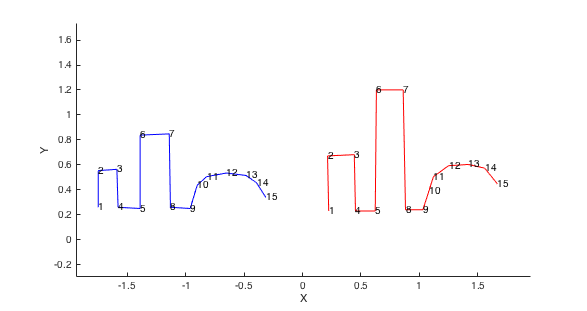
\includegraphics[width=1\linewidth]{./figures/similar_lines_A.png}
    \caption{Same direction \& rate (different scales)}
    \label{fig:similar_lines_A}
  \end{subfigure}
  \begin{subfigure}{.49\textwidth}
    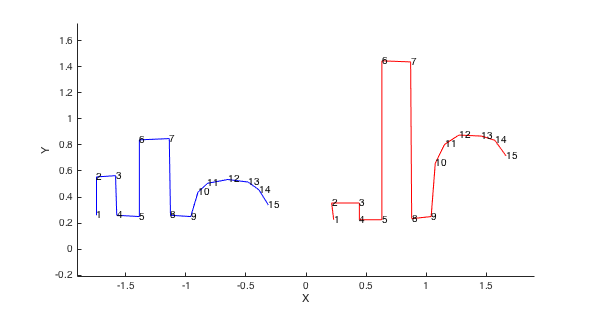
\includegraphics[width=1\linewidth]{./figures/similar_lines_B.png}
    \caption{Same direction but different rates}
    \label{fig:similar_lines_B}
  \end{subfigure}
  \begin{subfigure}{.49\textwidth}
    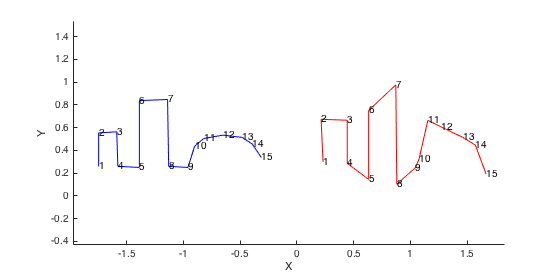
\includegraphics[width=1\linewidth]{./figures/similar_lines_C.png}
    \caption{Different directions}
    \label{fig:similar_lines_C}
  \end{subfigure}
  \caption{Lines of different similarity. From (a) to (c), shown in decreasing similarity.}
\end{figure}

Lines with complex curvatures can be expressed through series of points in Cartesian space. 
Affine transformations of scaling\eqref{eq:scale} and translation\eqref{eq:translate} produce new points defining lines who's coordinated are linearly related to the original. 
Pearson's correlation coefficient measures the extent to which two variables ($x_i$ and $x_i^\prime$) can be defined through a linear equation ($x_i^\prime = a * x_i + b$). \\
Correlation would therefore return high similarity if two lines are linear transformations of each other.    
\begin{equation}
  \begin{bmatrix}
    a_x & 0   & 0   \\
    0   & a_y & 0   \\
    0   & 0   &   1 \\ 
  \end{bmatrix} 
  *
  \begin{bmatrix}
    x_i \\ y_i \\ 1
  \end{bmatrix} 
  = 
  \begin{bmatrix}
    a_x * x_i \\ a_y * y_i \\ 1  
  \end{bmatrix}
  \label{eq:scale}
\end{equation}


\begin{equation}
  \begin{bmatrix}
    1 & 0 & b_x \\
    0 & 1 & b_y \\
    0 & 0 & 1   \\ 
  \end{bmatrix} 
  *
  \begin{bmatrix}
    x_i \\ y_i \\ 1
  \end{bmatrix} 
  = 
  \begin{bmatrix}
    x_i + b_x \\ y_i + b_y \\ 1  
  \end{bmatrix}
  \label{eq:translate}
\end{equation}

In the case of rotation\eqref{eq:rotate} or shearing\eqref{eq:shear}, the linear relationship between points is lost. 
Other transformations are combinations of  the above or deform shapes through distortion (e.g. barrel, pin cushion transformations) . 
For tool use scenarios involving rigid bodies only transition, scaling and rotation are realistic geometric transformations. 
Rotation is a common occurrence, and can be handled through PCA. 

\begin{equation}
  \begin{bmatrix}
    cos(\theta)  & -sin(\theta) &   0 \\
    -sin(\theta) & cost(\theta) &   0 \\
    	0   	 &	0       &   1 \\ 
  \end{bmatrix} 
  *
  \begin{bmatrix}
    x_i \\ y_i \\ 1
  \end{bmatrix} 
  = 
  \begin{bmatrix}
    x_i * cos(\theta) - y_i * sin(\theta) \\ x_i * sin(\theta) + y_i * cos(\theta) \\ 1
  \end{bmatrix} 
  \label{eq:rotate}
\end{equation}


\begin{equation}
  \begin{bmatrix}
    1 & h & 0 \\
    0 & 1 & 0 \\
    0 & 0 & 1   \\ 
  \end{bmatrix} 
  *
  \begin{bmatrix}
    x_i \\ y_i \\ 1
  \end{bmatrix} 
  = 
  \begin{bmatrix}
    x_i + h * y_i \\ y_i \\ 1  
  \end{bmatrix}
  \label{eq:shear}
\end{equation}

PCA returns a set of unit vectors that indicate the direction in which data has most variation. 
The rotation angle of a line can be removed by aligning the shape's principal components to the main X-Y axis.    
As affine rotations preserve variation, the principal vectors rotate by the same angles that a figure is rotated (figure \ref{fig:pca_rotation}).  

\begin{figure}[h]
  \centering
  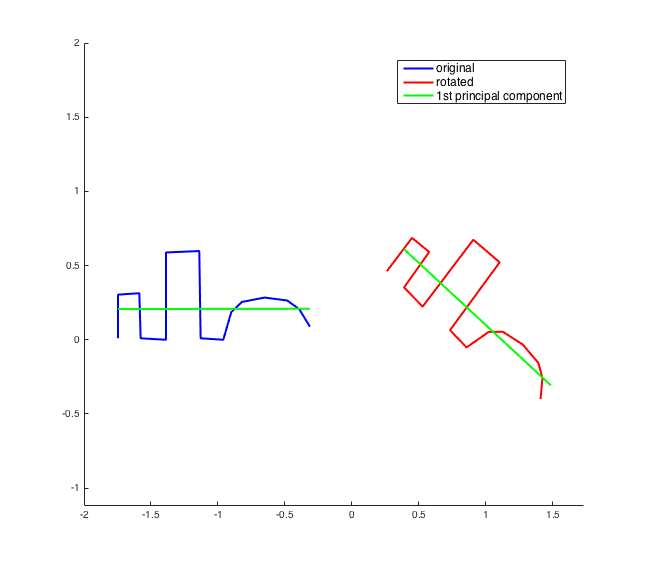
\includegraphics[width=.5\textwidth]{./figures/pca_rotation.png}
  \caption{First principal component rotating with the figure}
  \label{fig:pca_rotation}
\end{figure}  

Since principal components of a set of data are orthogonal, in the case of 2D data points, it is sufficient to align just the first principal component to the X axis.
Even in higher dimensionality of $n$ components, it is sufficient to align just the first $n-1$ components.

A rotation angle($\alpha$) can be retrieved from:
\begin{equation*}
\alpha = arctan(v_y,v_x)\ mod\ 2\pi 
\end{equation*}
Where $\vec{v}=(v_x,v_y)$ is the first principal component vector.

Using $\alpha$ all points defining a figure can be rotated in order to perform correlation. 
Similarity is calculated as the product of correlations over the individual X-Y coordinates.
Figures \ref{fig:correlation_2D} and \ref{fig:no_correlation_2D}, demonstrate the approach working on two hand drawn lines. 
Higher correlation is achieved for the more similar lines. 

\begin{figure}[h]
  \centering
  \begin{subfigure}{.5\textwidth}
    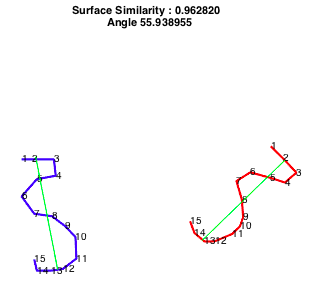
\includegraphics[width=1\linewidth]{./figures/correlation_2D.png}
    \caption{Similar contours}
    \label{fig:correlation_2D}
  \end{subfigure}
  \begin{subfigure}{.44\textwidth}
    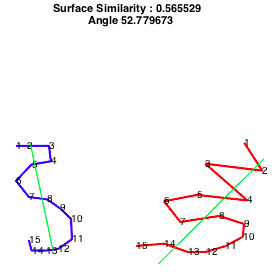
\includegraphics[width=1\linewidth]{./figures/no_correlation_2D.png}
    \caption{Dissimilar contours}
    \label{fig:no_correlation_2D}
  \end{subfigure}
  \caption{Comparison of simalirty measure}
\end{figure}

Correlation values are in the range of $[-1,+1]$, where:
\begin{itemize}
    \item values close to +1 represent high similarity
    \item values close to 0 represent dissimilarity 
    \item values close to -1 represent high similarity but mirrored (e.g. points are taken in reverse order) 
\end{itemize}

\pagebreak[2]
\subsubsection{3D case}

The components of the approach allow it to be applied to pairs of surfaces instead of lines. 
As with 2D shapes, points in 3D Cartesian space (i.e. X-Y-Z coordinates) can be organised in a grid structure defining a surface mesh (fig. \ref{fig:mesh_example}).

\begin{figure}[h]
  \centering
  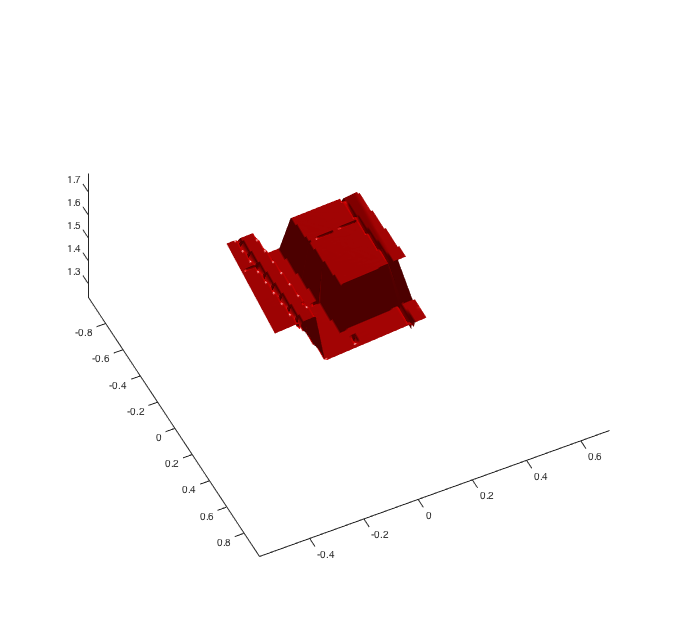
\includegraphics[width=.5\textwidth]{./figures/mesh_example.png}
  \caption{Example of surface mesh}
  \label{fig:mesh_example}
\end{figure}  

The similarity algorithm steps remain the same as in the 2D case: 
\begin{enumerate}
    \item Using PCA calculate the principal component vectors of each surface 
    \item Establish the rotation angles for aligning the first two principal component vectors to the X-Y axis 
    \item Rotate all point of the surfaces, using the established angles
    \item Calculate the product of correlations over all dimensions (i.e. X-Y-Z) 
\end{enumerate}

In 3D space, calculating angles and applying rotations involves different calculations.
Two angles($\alpha,\ \beta$) are required for aligning the first principal component vector against the X axis: 
\begin{equation*}
  \begin{split}
    \alpha = arctan(v_y^1,v_x^1)\ mod\ 2\pi\\
    \beta = -asin(v_z^1)\ mod\ 2\pi
  \end{split}
\end{equation*}
Where $\vec{v}_1=(v_x^1,v_y^1,v_z^1)$ is the direction vector of the first principal component.

The vector part of the second principal component must be rotated by $\alpha$ and $\beta$ in order to extract a third angle($\gamma$): 
\begin{equation*}
  \begin{split}
    v^2 = rotY(-\beta) * rotZ(-\alpha) * v^2\\
    \gamma = arctan(v_z^2,v_y^2)\ mod\ 2\pi 
  \end{split}
\end{equation*}
Where $\vec{v}_2=(v_x^2,v_y^2,v_z^2)$ is the direction vector of the second principal component and $rotY(-\beta)$ and $rotZ(-\alpha)$ are rotation matrices around the Y and Z axis.   

Surface points can then be aligned to the primary axes by multiplying them to the corresponding rotation matrices:  
\begin{equation*}
   P = rotX(-\gamma) * rotY(-\beta) * rotZ(-\alpha) * P
\end{equation*}
Where P is the set of points defining the surface mesh.

\subsubsection{Discussion}
The surface similarity technique, formally described, possesses the properties of effective contour matching techniques.
Translation and scaling invariance are immediate consequences of Pearson's correlation. 
Rotation invariance is attributed to  properties of PCA, allowing shapes to be aligned to the same orientation. 
Other non-linear transformations, such as shearing, added noise, or distortion would affect similarity measure proportional to the amount of applied deformation.    
These attributes place the technique as a potent candidate for most computer vision tasks.

Surface simulation can not be regarded as a global matching technique. 
Its strength lies in assessing part similarity, although it has no mechanism for determining the structure of a given shape.  
If shapes are prior decomposed into parts, the technique can be used in assessing individual parts. 

\begin{figure}[!h]
  \centering
  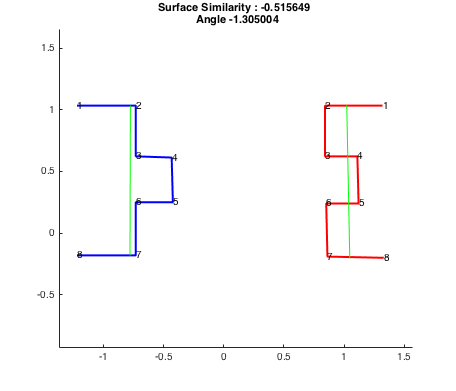
\includegraphics[width=.6\textwidth]{./figures/complementary.png}
  \caption{Complementary surfaces having negative similarity measure}
  \label{fig:complementary}
\end{figure}  

For the purpose of tool fitting, surface similarity carries additional helpful properties. 
The nature of tool use requires attention to complementary features rather than similar. 
Negative similarity measures would indicate complementary surfaces (fig. \ref{fig:complementary}). 
Care should be given as this property depends on the size of the visual field.
For example, in figure \ref{fig:complementary} if points 1 and 8 were removed, the surfaces would have 
a positive similarity value. 

Tool and object interaction require that intended parts are properly aligned.
Surface similarity can extract the necessary angle difference between complementary or similar shapes.
However, PCA orthogonal vectors are sometimes reversed, the resulting angle differences can occasionally be incorrect by $180^{\circ}$. 

Both complementarity and angle differences are highly desired traits for tool use problems.

In the case of tool use, the surface similarity algorithm can be computationally simplified.
Human subjects physically rotate objects so that important features face their perspective (fig. \ref{fig:same_orientation}). 
As such, analysed surfaces would have already aligned to the same orientation.
PCA rotations are therefore unnecessary in practice, and can lead to a simplified form of the algorithm.

\begin{figure}[!h]
  \centering
  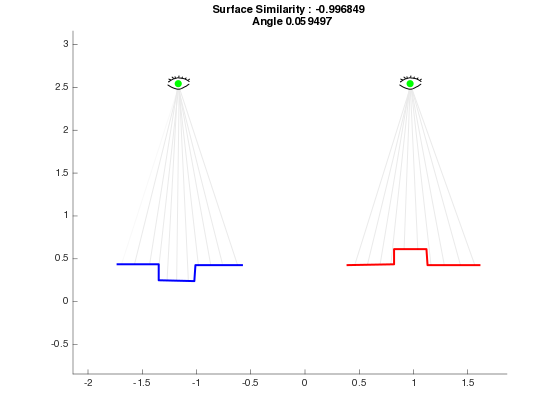
\includegraphics[width=.6\textwidth]{./figures/same_orientation.png}
  \caption{In practice, surfaces are already aligned to the user's point of view}
  \label{fig:same_orientation}
\end{figure}  

\begin{figure}[!h]
  \centering
  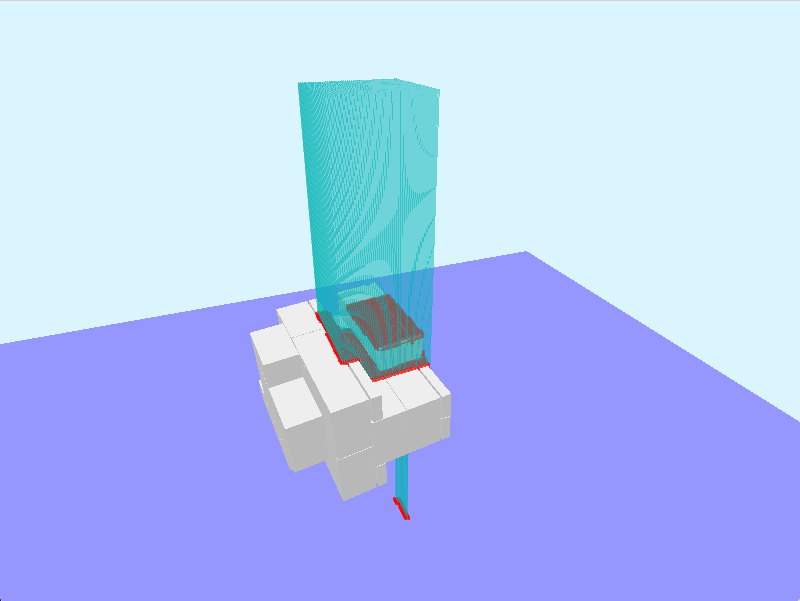
\includegraphics[width=.7\textwidth]{./figures/raycasting.png}
  \caption{Ray casting to extract surface points}
  \label{fig:raycasting}
\end{figure}  

\subsubsection{Evaluation}
The effectiveness of surface similarity was assessed using a physics simulator for a tool use scenario. 
Human depth perception and perspective was simulated through ray casting, by extracting object 3D surfaces. 
Ray casting is feature of physics engines which mimics the propagation of light. 
Surface are extracted by casting a grid of parallel rays over an object model as in figure \ref{fig:raycasting}). 

\begin{figure}[!h]
  \centering
  \begin{subfigure}{1\textwidth}
    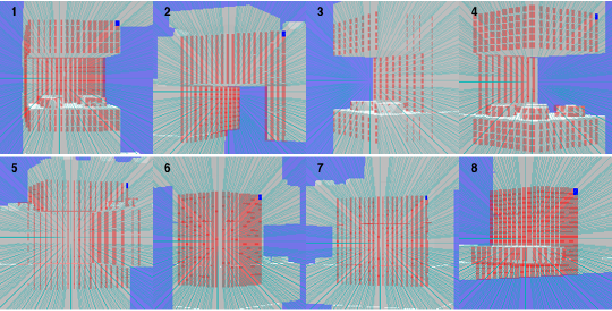
\includegraphics[width=1\linewidth]{./figures/object_parts.png}
    \caption{Object surfaces}
    \label{fig:obj_parts}
  \end{subfigure}
  \begin{subfigure}{1\textwidth}
    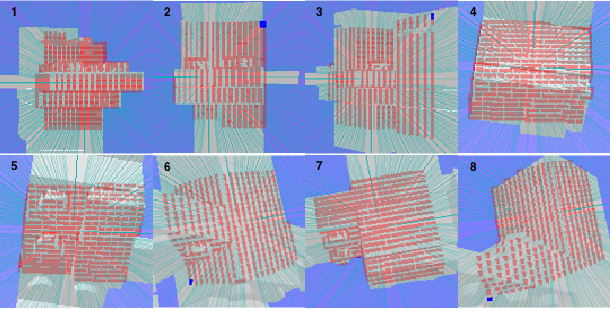
\includegraphics[width=1\linewidth]{./figures/tool_parts.png}
    \caption{Tool surfaces}
    \label{fig:tool_part}
  \end{subfigure}
  \caption{Surfaces extracted from both tool and object}
\end{figure}

A first test verifies the effectiveness of the algorithm and the impact of PCA to the similarity measures. 
$8$ pairs of tool and object surfaces were extracted (fig. \ref{fig:obj_parts},\ref{fig:tool_part}). 
The first set of $4$, were chosen to represent parts that are of interest to human subjects. 
A second set have no tool fitting value. 
Figure \ref{fig:correlation_parts} shows a grid of correlation values for each combination of surfaces. 
In either the PCA or simplified form, the algorithm returns complementary matching for pairs in the first set of surfaces. 
Other combination achieve 0 or positive similarity, making them less possible tool fitting candidates. 
The results match intuition of object parts that would provide good fitting. 

\begin{figure}[!h]
  \centering
  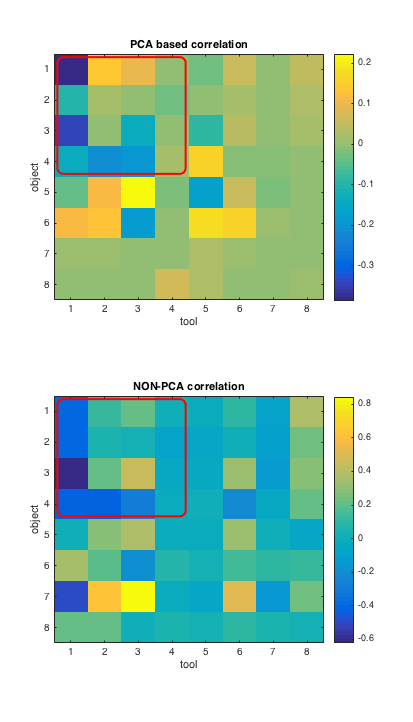
\includegraphics[width=0.8\textwidth]{./figures/correlation_comparison.png}
  \caption{Complementary correlation occurs mostly between parts of interest}
  \label{fig:correlation_parts}
\end{figure}  

It is worth observing that a non-PCA algorithm tends to return more false positive matches. 
Yet, because of its reduced complexity, we employ the simplified algorithm in a heuristic visual search implementation.

As previously mentioned,tool and object fitting can be optimised by visually detecting compatible parts.  
Visual search simulates the act of finding potential solutions inside the physics simulator.
Given a tool and object, the search randomly selects surfaces to assesses complementarity.
When a pair is found, the simulation pauses and lets a human assessor verify validity (fig. \ref{fig:visual_search}). 

\begin{figure}[!h]
  \centering
  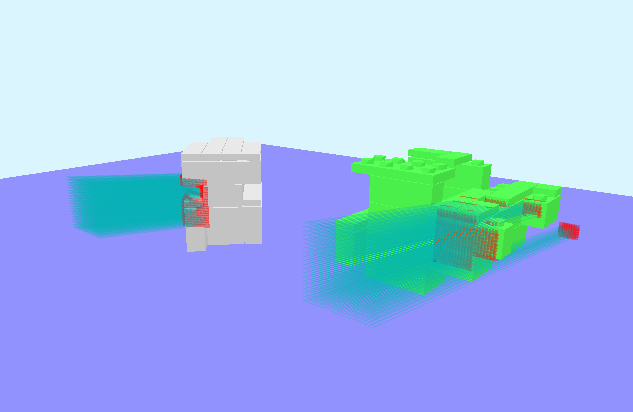
\includegraphics[width=0.8\textwidth]{./figures/visual_search.png}
  \caption{Complementary surfaces found by visual search}
  \label{fig:visual_search}
\end{figure}  

Due to project time constraints the effectiveness of visual search was not formally assessed. 
Future investigation will have to compare results to human data, potentially carrying eye tracking information. 

Additionally, further improvements can be made to the implementation:
\begin{enumerate}
   \item The search contains no strategy to decompose objects into parts 
   \item Ideally, sub-regions of similarity should be located within larger surfaces 
   \item The size of analysed surfaces was arbitrarily chosen and can be adjusted for better results  
   \item Matched surfaces should be verified by fitting the tool and object 
   \item The PCA based algorithm can be used to remove false positive results 
\end{enumerate}

\printbibliography 

\end{document}
